\documentclass[10pt, letterpaper]{article}
\usepackage[cm]{fullpage}
\usepackage{algpseudocode}
\usepackage{algorithm}
\usepackage{graphicx}
\usepackage[section]{placeins}
\usepackage[table]{xcolor}
\usepackage{amsmath}
\usepackage[margin=0.7in]{geometry}

\algrenewcommand\Return{\State \algorithmicreturn{} }%

\title{0-1 Knapsack}
\author{Daiwei Chen \and Joseph Watts}
\date{\today}

\begin{document}
\maketitle
\begin{abstract}
	0-1 Knapsack is the coined phrase which is used to simply describe the problem of finding the maximum value possible by choosing what items to take, when not everything can be taken.
 Put slightly more formally, given a set of items with all items having a value and weight assigned to them and a bag which allows the user to carry unlimited volume but only a limited weight, the goal is to find the set of items which allow the user to get the maximum value from the chosen items.
This paper explores different approaches to solving this problem including both a Dynamic Programming approach along with multiple different Greedy approaches.

\end{abstract}

\section{Background and Related Work}
In the year 2000, the Y2K bug destroyed all computer software worldwide. Millions of computer scientists lost their jobs in the catastrophy. Many of these computer scientists turned towards becoming a thief as the alternative occupation. Somehow, many of these computer scientists got themselves a very, very large bag. An bag of infinite size if you will. Unfortunately, due to long days of sitting still, many of these computer scientists can only carry so much. Thus comes the question, how do you determine which items to steal at an efficient manner to obtain the most value for the amount of weight you can carry. And what's the best way to figure out a solution (fastest solution vs. best solution, or both)?\\
\\
The Knapsack problem relates very closely to anything that requires resource allocation. In many problems, one of the largest constraits is resources, be it time, money, or talent. To be more efficient, it's important for anyone to use the resources they have to achieve the greatest result possible.\\
\\
The 0-1 Knapsack problem is commonly found in project management and economics in dealing with resource allocation. In an oversimplified manner, how can resources divided so that different departments can get the most valuable work done given their needed resources.
0-1 Knapsack also shows up when working with networking equiptment which try to most efficiently distribute load between different stations.
This is known as load balancing and is used in many common day-to-day technologies.
0-1 Knapsack was also used as a key part of the design of public-private keys when first made during the 1970's. A private key is generated with an easy knapsack problem, and then a hard knapsack is derrived by it and this is what is used as the public key.

\section{Greedy Algorithm}

\begin{algorithm}
  \begin{algorithmic}
    \caption{GreedyGrab}\label{GreedyGrab}
    \Function{GreedyGrab}{items, maxWeight}
    \State total $\gets$ 0
    \For{item in items}
    \If{item.weight $\leq$ maxWeight}
    \State maxWeight $\gets$ maxWeight - item.weight
    \State total $\gets$ total + item.value
    \EndIf
    \If{maxWeight $=$ 0}
    \Return total
    \EndIf
    \EndFor
    \Return total
    \EndFunction
  \end{algorithmic}
\end{algorithm}


\section{Dynamic Algorithm}
\begin{algorithm}
	\begin{algorithmic}
		\caption{DynAlgo}\label{DynAlgo}
		\Function{DynAlgo}{items, maxWeight}
		\State n $\gets$ len(items)
		\For{i in range(n)}
			\For{j in range(maxWeight + 1)}
				\State table[i][0] $\gets$ 0
				\If{j $<$ items[0].weight}
					\State table[0][j] $\gets$ 0
				\EndIf
				\If{j $\geq$ items[0].weight}
					\State table[i][j] $\gets$ max(table[i-1][j], table[i-1][j-items[i].weight] + items[i].value)
				\EndIf
			\EndFor
		\EndFor
		\Return table[n-1][maxWeight]
		\EndFunction
	\end{algorithmic}
\end{algorithm}

This dynamic programming solution builds a table of size $n$ by $W+1$ where $n$ is the number of available items, and $W$ is the maximum weight that is available. For each row, $i$, and each column, $j$,  set that row's first column equal to zero. If $j$ is less than the first item in the item list's weight then set the first row's column at $j$ equal to the value of the first item in the item's list.
Now that the first row and column have been populated, the remaining elements can also be calculated.
If $j$ is less than the current item's weight, then the current row and column's value is set to the value held at the the previous row and the current column. Otherwise the value found at the current row and column is set as the maximum between the value at the previous row and current column and the value found at the prevoius row and current column minus the current items weight. This is in addition to the current items value. The optimal value can now be read at K[$n-1$][$W$]


\medskip
While at first glance it may appear that this algorithm will run in $\theta(n^2)$ time, it actually depends on both the number of items that are available, and the maximum weight allowed, which changes the number of items that you get to choose from. This leads this dynamic algorithm to have $\theta(n * W)$ complexity where $n$ is the number of available items and $W$ is the maximum weight.
\section{Experimental Setup}
This experiment was setup to run 100 trials of calculations. 100 items with a value between 1 and 25 were generated all having a weight between 1 and 10. Between each run of the experiment the maximum weight was increased by 100, up to 500. Timings were one for the Dynamic Algorithm and three Greedy approaches: increasing weight, decreasing value, and decreasing ratio (value/weight). Accuracy for these were also compared to dynamic programming and calculated as a \% of the optimal answer. All times were recorded in nanoseconds with Python on an Intel i5-2520m with 16gb of ddr3 memory running Ubuntu 18.10 as its operating system. 5.0.1-050001-generic was the kernel of choice.
\section{Results}
	% Diagram showing the average time between different approaches
	\begin{figure}[htbp]
		\begin{center}
			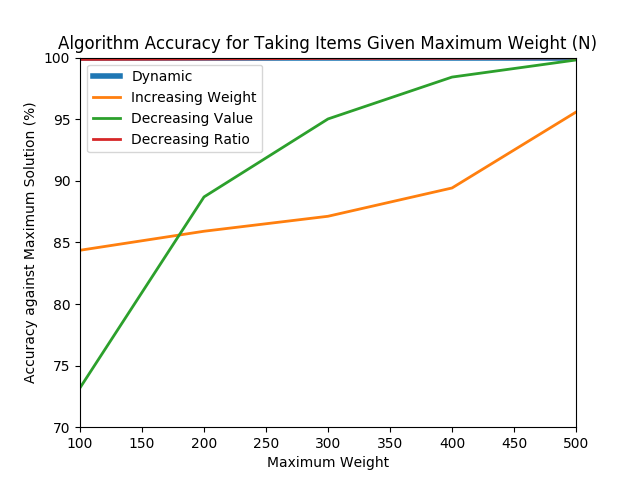
\includegraphics[width=0.70\textwidth]{python/accuracyGraph.png}
			\caption{Algorithm Accuracy for Taking Items Given Maximum Weight $n$}
			\label{fig:accuracy-graph}
		\end{center}
	\end{figure}
	% Diagram showing the % accuracy of different approaches
	\begin{figure}[htbp]
		\begin{center}
			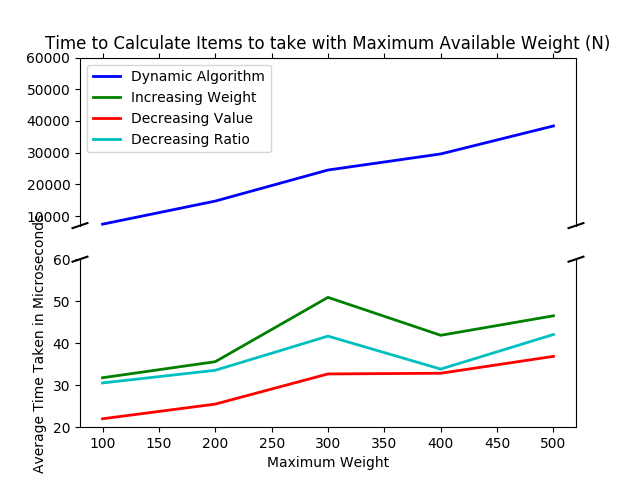
\includegraphics[width=0.70\textwidth]{python/timeGraph.png}
			\caption{Time to Calculate Items to take with Maximum Available Weight $n$}
			\label{fig:time-graph}
		\end{center}
	\end{figure}

\section{Conclusions}


\end{document}
